\documentclass{beamer}[10]

\usepackage{graphicx}
\usepackage{xcolor}
\usepackage{tabto}
%\usepackage{beamerthemesplit}
\usepackage{tikz}
\usepackage{cancel}
\usepackage{verbatim}
\usepackage{fancybox}
\usepackage{enumerate}
\usepackage{amsmath,amssymb,amsthm,textcomp,mathtools}
\usepackage[super]{nth}
\usepackage[amssymb]{SIunits}
\usepackage{booktabs}
\usepackage{cancel}
\usepackage{bm}
\usepackage[utf8]{inputenc}
\usepackage{tabularx}
\usepackage{ragged2e}
\newcolumntype{Y}{ >{\RaggedRight\arraybackslash}X}
\usetikzlibrary{arrows,shapes}
\newcommand\T{\rule{0pt}{2.6ex}}
\newcommand\B{\rule[-1.2ex]{0pt}{0pt}}
\definecolor{UUcrimson}{RGB}{204,0,0}
\mode<presentation>
{ \usetheme{default}
  \usecolortheme[named=UUcrimson]{structure}
  \useinnertheme{circles}
  \setbeamercovered{transparent}
  \setbeamertemplate{blocks}[rounded]
  \usefonttheme[onlymath]{serif}
  \setbeamertemplate{navigation symbols}{}
  \setbeamertemplate{footline}[page number]
  \setbeamertemplate{navigation symbols}{}
  \setbeamercolor{section in toc}{fg=black,bg=white}
  \setbeamercolor{alerted text}{fg=UUcrimson!80!gray}
  \setbeamercolor*{palette primary}{fg=white,bg=UUcrimson}
  \setbeamercolor*{palette secondary}{fg=UUcrimson!70!black,bg=gray!15!white}
  \setbeamercolor*{palette tertiary}{bg=UUcrimson!80!black,fg=gray!10!white}
  \setbeamercolor*{palette quaternary}{fg=UUcrimson,bg=gray!5!white}
  \setbeamercolor*{palette sidebar primary}{fg=UUcrimson!10!black}
  \setbeamercolor*{palette sidebar secondary}{fg=white}
  \setbeamercolor*{palette sidebar tertiary}{fg=UUcrimson!50!black}
  \setbeamercolor*{palette sidebar quaternary}{fg=gray!10!white}
  \setbeamercolor{titlelike}{parent=palette primary,fg=white}
  \setbeamercolor{frametitle}{bg=UUcrimson}
  \setbeamercolor{frametitle right}{bg=UUcrimson}
  \setbeamercolor*{separation line}{}
  \setbeamercolor*{fine separation line}{}
}

\usetikzlibrary{backgrounds}
\makeatletter
\tikzstyle{every picture}+=[remember picture]
\tikzset{%
  fancy quotes/.style={
    text width=\fq@width pt,
    align=justify,
    inner sep=1em,
    anchor=north west,
    minimum width=\linewidth,
    font=\itshape
  },
  fancy quotes width/.initial={.8\linewidth},
  fancy quotes marks/.style={
    scale=8,
    text=white,
    inner sep=0pt,
  },
  fancy quotes opening/.style={
    fancy quotes marks,
  },
  fancy quotes closing/.style={
    fancy quotes marks,
  },
  fancy quotes background/.style={
    show background rectangle,
    inner frame xsep=0pt,
    background rectangle/.style={
      fill=gray!25,
      rounded corners,
    },
  }
}
\newenvironment{fancyquotes}[1][]{%
\noindent
\tikzpicture[fancy quotes background]
\node[fancy quotes opening,anchor=north west] (fq@ul) at (0,0) {``};
\tikz@scan@one@point\pgfutil@firstofone(fq@ul.east)
\pgfmathsetmacro{\fq@width}{\linewidth - 2*\pgf@x}
\node[fancy quotes,#1] (fq@txt) at (fq@ul.north west) \bgroup}
{\egroup;
\node[overlay,fancy quotes closing,anchor=east] at (fq@txt.south east) {''};
\endtikzpicture}
\makeatother

\usepackage{scalerel}[2014/03/10]
\usepackage{stackengine}
\usepackage{empheq}
\newcommand*\widefbox[1]{\fbox{\hspace{0.5em}#1\hspace{0.5em}}}

\newcommand\reallywidetilde[1]{\ThisStyle{%
  \setbox0=\hbox{$\SavedStyle#1$}%
  \stackengine{-.1\LMpt}{$\SavedStyle#1$}{%
    \stretchto{\scaleto{\SavedStyle\mkern.2mu\sim}{.5467\wd0}}{.4\ht0}%
%    .2mu is the kern imbalance when clipping white space
%    .5467++++ is \ht/[kerned \wd] aspect ratio for \sim glyph
  }{O}{c}{F}{T}{S}%
}}
\usepackage{media9}

\logo{
\includegraphics[width=0.75cm]{logo.jpg}}
\author[Gibbs]{Dr. Jeremy A. Gibbs}
\institute{Department of Mechanical Engineering\\University of Utah}
\date{Fall 2016}
\title{LES of Turbulent Flows: Lecture 5}

\begin{document}

%----------------------------------------------------------------------------------------
%	TITLE & TOC SLIDES
%----------------------------------------------------------------------------------------

\begin{frame} 
  \titlepage
\end{frame}

%------------------------------------------------

\begin{frame}
\frametitle{Overview}
\tableofcontents
\end{frame}

%------------------------------------------------
\section{Recap of N-S equations} %
%------------------------------------------------
\begin{frame}{Recap}

\begin{itemize}
	\item The Navier-Stokes equations describe the motion of fluids, through the conservation of mass, momentum, and energy.
	\item The equations are nonlinear, which complicates our ability to analyze and simulate fluid flows.
	\item Why? The nonlinearity creates a continuous spectrum of different flow features.
\end{itemize}

\end{frame}


%------------------------------------------------

\begin{frame}{Recap of N-S equations}

\begin{itemize}
	\item This spectrum contains very large integral scales and very small dissipation scales.
	\item The simultaneous representation of both large and small scales makes for a very large computational problem.
	\item Current computational resources limit the amount of small features that can be accurately simulated.
\end{itemize}
\end{frame}

%------------------------------------------------

\begin{frame}{Recap}

\begin{itemize}
	\item The complexity of a flow can be reduced to alleviate this computation bottleneck.
	\item This technique is aimed at capturing the primary features of a flow with sufficient detail and accepting that the full turbulent solution may not be obtained perfectly.
	\item This sets the stage for LES as a tool to solve for the ``reduced'' flow.
	\item Before diving into LES, we will go over the description of the DNS, LES, and RANS techniques.
\end{itemize}
\end{frame}

%------------------------------------------------
\section{Approximating the equations of motion} %
%------------------------------------------------
\begin{frame}{Approximating the equations of motion}

\begin{itemize}
	\item Numerical studies require that the equations of motion for a (compressible, incompressible, Boussinesq) fluid must be approximated on a computational grid using discrete physical points or basis functions.
	\item Three basic methodologies are prevalent in turbulence application and research:
	\begin{itemize}
		\item Direct Numerical Simulation (DNS)
		\item Large-Eddy Simulation (LES)
		\item Reynolds-Averaged Navier-Stokes (RANS)
	\end{itemize}
\end{itemize}
\end{frame}

%------------------------------------------------

\begin{frame}{Approximating the equations of motion}

Direct Numerical Simulation
\begin{itemize}
	\item The DNS approach focuses on finding a numerically-accurate solution to the N-S equations (\textit{i.e.}, resolve all eddies).
	\item As we saw last class, it is an expensive operation.
\end{itemize}
\end{frame}

%------------------------------------------------

\begin{frame}{Approximating the equations of motion}

Large-Eddy Simulation
\begin{itemize}
	\item The LES approach emphasizes capturing those primary flow features that are larger than a prescribed filter width ($\Delta$) (\textit{i.e.}, resolve larger-eddies and model smaller ``universal'' ones).
	\item Since $\Delta$ is prescribed, one has control over the required resolution and computational effort.
	\item The LES approach introduces the closure problem and reduces the information of the resolved flow.
	\item Has primarily trended toward engineering applications, but its use in atmospheric science is increasing.
\end{itemize}

\end{frame}

%------------------------------------------------

\begin{frame}{Approximating the equations of motion}

Reynolds-Averaged Navier-Stokes
\begin{itemize}
	\item The RANS approach focuses on a statistical description of the basic fluctuation-correlations (\textit{i.e.}, model ensemble statistics).
	\item Can be used to study flows with realistic complexity.
\end{itemize}
\end{frame}

%------------------------------------------------

\begin{frame}{Approximating the equations of motion}
\begin{figure}
	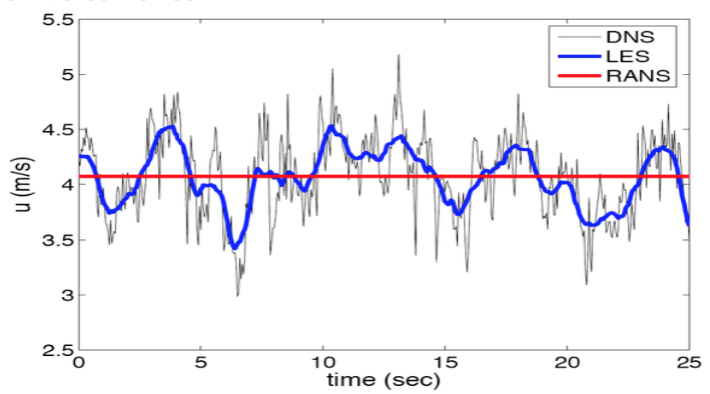
\includegraphics[width=\textwidth]{methods1.png}
\end{figure}
\end{frame}


%------------------------------------------------
\section{Pros and cons of each method} %
%------------------------------------------------
\begin{frame}{Pros and cons of each method}

Direct Numerical Simulation
\begin{itemize}
	\item Pros
	\begin{itemize}
		\item Does not require the use of a turbulence model
		\item Accuracy is only limited by computational capabilities since errors are generally only due to sensitivity to perturbations or accumulated round-off errors.
		\item All aspects of the flow in time and space are available, which is not possible for experiments (\textit{i.e.}, 3D velocity and scalar fields).
	\end{itemize}

\end{itemize}
\end{frame}

%------------------------------------------------
\begin{frame}{Pros and cons of each method}

Direct Numerical Simulation
\begin{itemize}
	\item Cons
	\begin{itemize}
		\item Restricted to low-Re flows with relatively simple geometries.
		\item Very high memory and computational time costs.
		\item Typically the ``largest possible'' number of grid points is used without proper convergence evaluation (\textit{i.e.}, does not allow for systematic variation of numerical and physical parameters)
	\end{itemize}
\end{itemize}
\end{frame}

%------------------------------------------------

\begin{frame}{Pros and cons of each method}

Large-Eddy Simulation
\begin{itemize}
	\item Pros
	\begin{itemize}
		\item Only small scales require require modeling. Since the small scales are likely insensitive to specifics of the flow, these models can be rather simple and ``universal''.
		\item Much cheaper computational cost than DNS.
		\item Unsteady predictions of the flow are made, which implies that information about extreme events are available over some period of time.
		\item Properly designed LES should allow for $Re\Rightarrow\infty$.
		\item In principle, we can gain as much accuracy as desired by refining our numerical grid.
	\end{itemize}

\end{itemize}
\end{frame}

%------------------------------------------------

\begin{frame}{Pros and cons of each method}

Large-Eddy Simulation
\begin{itemize}
	\item Cons
	\begin{itemize}
		\item Basic assumption (small scales are universal) requires independence of small (unresolved) scales from boundary conditions (especially important for flow geometry). This is a problem for boundary layers, where proximity to the wall defines some of the smallest scales of the flow -- which necessitates explicit modeling of the region.
		\item Still very costly for many practical engineering applications.
		\item Filtering and turbulence theory of small scales still needs development for complex geometry and highly anisotropic flows.
	\end{itemize}

\end{itemize}
\end{frame}

%------------------------------------------------

\begin{frame}{Pros and cons of each method}

Reynolds-Averaged Navier-Stokes
\begin{itemize}
	\item Pros
	\begin{itemize}
		\item Low computational cost (can obtain mean statistics in a short time).
		\item Can be used for highly complex flow geometries.
		\item When combined with empirical information, can be highly useful for engineering applications and to parameterize near-wall behavior.
	\end{itemize}

\end{itemize}
\end{frame}

%------------------------------------------------

\begin{frame}{Pros and cons of each method}

Reynolds-Averaged Navier-Stokes
\begin{itemize}
	\item Cons
	\begin{itemize}
		\item Only steady flow phenomena can be explored with full advantage of computational reduction.
		\item Models are not universal since dynamic consequences of all scales must be represented. Usually a pragmatic ``tuning'' of model parameters is required for specific applications.
		\item Most accurate turbulence models give rise to highly complex equations sets, which can lead to numerical formulation and convergence issues.
	\end{itemize}

\end{itemize}
\end{frame}

%------------------------------------------------

\begin{frame}{Relationship between each method}

\begin{itemize}
	\item DNS delivers the most accurate data (in general).
	\item DNS can be used to validate and analyze aspects of LES, such as numerical methods and subgrid model.
	\item LES provides a more complete picture of turbulent flow than RANS.
	\item RANS can be validated against LES data (where LES is used to obtain statistical information about the flow).
\end{itemize}
\end{frame}

%------------------------------------------------

\begin{frame}{Relationship between each method}

\begin{figure}
	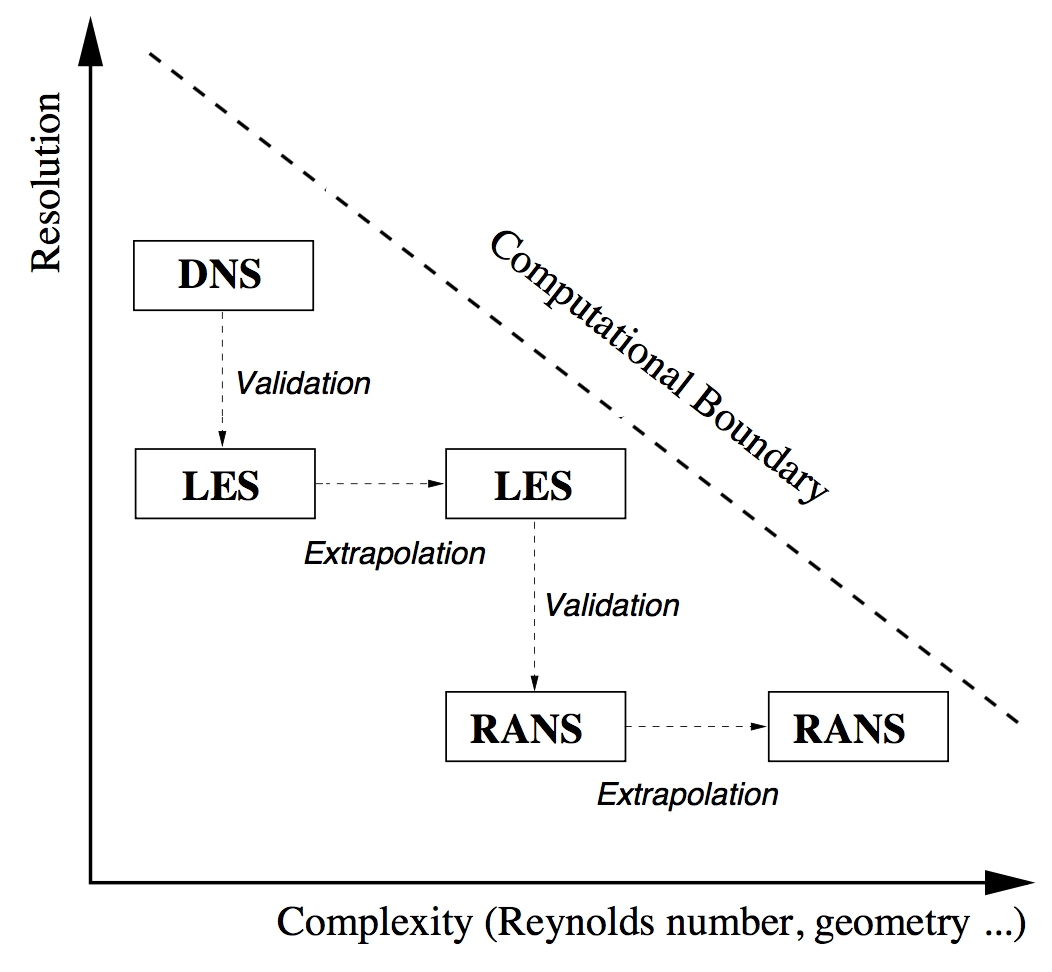
\includegraphics[width=0.8\textwidth]{methods2.png}
\end{figure}

\end{frame}

%------------------------------------------------
\section{Scale separation} %
%------------------------------------------------
\begin{frame}{Scale separation}

\begin{itemize}
	\item So far, we have discussed LES very generically:
	\begin{itemize}
		\item Resolve only the largest energy-containing scales.
		\item Model the small ``universal'' scales.
	\end{itemize}
	\item We will now formalize the idea of scale separation mathematically to show how to deal with the equations of motion and derive subgrid models.

\end{itemize}
\end{frame}

%------------------------------------------------
\begin{frame}{Scale separation}

\begin{itemize}
	\item How do we accomplish scale separation?
	\begin{itemize}
		\item A \textbf{low-pass filter}
	\end{itemize}
	\item What is meant by \textit{low-pass}?
	\begin{itemize}
		\item A low-pass filter \textit{passes} over signals with a frequency (wavenumber) \textit{lower} than a certain cutoff frequency (wavenumber) and only smooths signals with a frequency (wavenumber) higher than the cutoff value.
	\end{itemize}
	\item Our goal for the low-pass filter:
	\begin{itemize}
		\item Attenuate (smooth) \textbf{high frequency} (high wavenumber/small scale) turbulence features that are smaller than a prescribed characteristic scale $\Delta$ while leaving \textbf{low-frequency} (low wavenumber/large scale) motions unchanged. 
	\end{itemize}
\end{itemize}
\end{frame}

%------------------------------------------------
\begin{frame}{Filtering}

\textbf{\underline{Filtering}} (Sagaut Chapter 2, Pope Chapter 13.2)
\begin{itemize}
	\item The formal (mathematical) LES filter is a convolution filter defined for a quantity $\phi (\vec{x},t)$ in physical space as:
	$$\tilde \phi (\vec{x},t) = \int_{-\infty}^{\infty} \phi (\vec{x} - \vec{\zeta},t) G(\vec{\zeta}) d \vec{\zeta}$$
	\item $G \equiv$ the convolution kernel of the chosen filter.
	\item $G$ is associated with the characteristic cutoff scale $\Delta$ (also called the filter width).
\end{itemize}
\end{frame}

%------------------------------------------------
\begin{frame}{Convolution}

\begin{itemize}
	\item So, we have the convolution filter 
	$$\tilde \phi (\vec{x},t) = \int_{-\infty}^{\infty} \phi (\vec{x} - \vec{\zeta},t) G(\vec{\zeta}) d \vec{\zeta}$$
	\item Here we will use Pope's notation for the Fourier transform:
	$$F\{\phi(x)\} = \int_{-\infty}^{\infty} e^{-ikx}\phi(x)dx$$
\end{itemize}
\end{frame}

%------------------------------------------------
\begin{frame}{Convolution}

\begin{itemize}
	\item Take the Fourier transform of $\tilde \phi (\vec{x})$ (dropping $t$ for simplicity):
	$$F\{\tilde \phi(\vec{x})\} = \int_{-\infty}^{\infty} e^{-i\vec{k}\vec{x}} \int_{-\infty}^{\infty} \phi (\vec{x} - \vec{\zeta},t) G(\vec{\zeta}) d \vec{\zeta} d \vec{x}$$
	\item We can define a new variable $\vec{r} = \vec{x} - \vec{\zeta}$:
	\begin{align*}
	F\{\tilde \phi(\vec{x})\} &= \int_{-\infty}^{\infty} e^{-i\vec{k}(\vec{r} + \vec{\zeta})} \int_{-\infty}^{\infty} \phi(\vec{r}) G(\vec{\zeta}) d\vec{\zeta} d\vec{r}\\
	&= \int_{-\infty}^{\infty} \int_{-\infty}^{\infty} e^{-i\vec{k}(\vec{r} + \vec{\zeta})} \phi(\vec{r}) G(\vec{\zeta}) d\vec{\zeta} d\vec{r}
	\end{align*}
	Note: $d\vec{r} = d\vec{x}$ because $\vec{\zeta} \neq f(\vec{x})$ and we changed the order of integration
\end{itemize}
\end{frame}

%------------------------------------------------
\begin{frame}{Convolution}

\begin{itemize}
	\item We left off with: $$F\{\tilde \phi(\vec{x})\}= \int_{-\infty}^{\infty} \int_{-\infty}^{\infty} e^{-i\vec{k}(\vec{r} + \vec{\zeta})} \phi(\vec{r}) G(\vec{\zeta}) d\vec{\zeta} d\vec{r}$$
	\item Recall that $e^{a+b} = e^a e^b$:
	\begin{align*}
	F\{\tilde \phi(\vec{x})\} &= \int_{-\infty}^{\infty} \int_{-\infty}^{\infty} e^{-i\vec{k}\vec{r}} e^{-i\vec{k}\vec{\zeta}} \phi(\vec{r}) d\vec{r}  G(\vec{\zeta}) d\vec{\zeta}\\
	&= \int_{-\infty}^{\infty} e^{-i\vec{k}\vec{r}} \phi(\vec{r}) d\vec{r} \int_{-\infty}^{\infty} e^{-i\vec{k}\vec{\zeta}} G(\vec{\zeta}) d\vec{\zeta}\\
	\Aboxed{&= F\{\phi(\vec{x})\}F\{G(\vec{\zeta})\}}
	\end{align*}
	where we changed the order for integration
\end{itemize}
\end{frame}

%------------------------------------------------
\begin{frame}{Convolution}

\begin{itemize}
	\item We found this convolution relationship:
	$$\boxed{F\{\tilde \phi(\vec{x})\} = F\{\phi(\vec{x})\}F\{G(\vec{\zeta})\}}$$
	\item Segaut writes this as:
	$$\tilde{\hat \phi}(\vec{k},\omega) = \hat \phi(\vec{k},\omega)\hat G(\vec{k}\omega)$$
	where ($\ \hat{ }\ $) denotes a Fourier coefficient.
\end{itemize}
\end{frame}

%------------------------------------------------
\begin{frame}{Convolution}

\begin{itemize}
	\item $F\{\tilde \phi(\vec{x})\} = F\{\phi(\vec{x})\}F\{G(\vec{\zeta})\}$ or $\tilde{\hat \phi}(\vec{k},\omega) = \hat \phi(\vec{k},\omega)\hat G(\vec{k}\omega)$
	\item $\hat G$ is the transfer function associated with the filter kernel $G$.
	\item Recall, that a transfer function is the wavespace (Fourier) relationship between the input and output of a linear system.
	\item A convolution is an integral that expresses the amount of overlap of one function $G$ as it is shifted over another function $\phi$ (\textit{i.e.}, it blends one function with another).
\end{itemize}
\end{frame}

%------------------------------------------------
\begin{frame}{Decomposition into resolved and subfilter components}

\begin{itemize}
	\item Just as $G$ is associated with a filter scale $\Delta$ (filter width), $\hat G$ is associated with a cutoff wavenumber  $k_c$.
	\item In a similar manner to Reynolds decomposition, we can use the filter function to decompose the velocity field into resolved and unresolved (or subfilter) components:
	$$\underbrace{\phi(\vec{x},t)}_{\text{total}} = \underbrace{\tilde \phi (\vec{x},t)}_{\text{resolved}} + \underbrace{\phi^{\prime}(\vec{x},t)}_{\text{subfilter}}$$
\end{itemize}
\end{frame}

%------------------------------------------------
\begin{frame}{Fundamental properties of ``proper'' LES filters}

\begin{itemize}
	\item The filter should not change the value of a constant $a$
	$$\int_{-\infty}^{\infty} G(\vec{x})d\vec{x} = 1 \Rightarrow \tilde a = a$$
	\item Linearity $$\widetilde{\phi + \zeta} = \tilde \phi + \tilde \zeta$$
	(this is automatically satisfied for a convolution filter)
	\item Commutation with differentiation
	$$\frac{\widetilde{\partial \phi}}{\partial \vec{x}} = \frac{\partial \tilde \phi}{\partial \vec{x}}$$
\end{itemize}
\end{frame}

%------------------------------------------------
\begin{frame}{LES and Reynolds Operators}

\begin{itemize}
	\item In the general case, LES filters that verify these properties are not Reynolds operators.
	\item Recall for a Reynolds operator (average) defined by $\langle \ \rangle$
	\begin{itemize}
		\item $\langle a\phi\rangle = a\langle \phi \rangle$
		\item $\langle \phi^\prime \rangle = 0$
		\item $\langle \phi + \zeta \rangle = \langle \phi \rangle + \langle \zeta \rangle$
		\item $\langle \langle \phi \rangle \rangle = \langle \phi \rangle$
		\item $\langle \cfrac{\partial \phi}{\partial \vec{x}}\rangle = \cfrac{\partial \langle \phi \rangle}{\partial \vec{x}}$	
	\end{itemize}
\end{itemize}
\end{frame}

%------------------------------------------------
\begin{frame}{LES and Reynolds Operators}

\begin{itemize}
	\item For our LES filter, in general using Sagaut's shorthand $\int_{-\infty}^{\infty} \phi(\vec{r},t)G(\vec{\zeta}) d\vec{\zeta} = G \star \phi$:
	\begin{itemize}
		\item $\tilde{\tilde \phi} = G \star G \star \phi = G^2 \star \phi \neq \tilde \phi = G \star \phi$
		\item $\tilde \phi^{\prime} = G \star (\phi - G \star \phi) \neq 0$
	\end{itemize}
	\item For an LES filter, a twice filtered variable is not equal to a single filtered variable -- unlike it is for a Reynolds average.
	\item Likewise, the filtered subfilter scale component is not equal to zero as it is for a Reynolds average.
\end{itemize}
\end{frame}

%------------------------------------------------
\begin{frame}{Common (or classic) LES filters}

\begin{itemize}
	\item Box or ``top-hat'' filter (equivalent to a local average):
	$$\underbrace{G(r) = \begin{cases} \frac{1}{\Delta} &\mbox{if } r \leq \frac{\Delta}{2} \\ 0 & \mbox{otherwise }\end{cases}}_{\text{filter function}} \qquad \underbrace{\vphantom{\begin{cases} \frac{1}{\Delta} &\mbox{if } \vec{r} \leq \frac{\Delta}{2} \\ 0 & \mbox{otherwise }\end{cases}} \hat G(k) = \frac{\sin{(k\Delta/2)}}{k\Delta/2}}_{\text{transfer function}}$$
	\item Gaussian filter ($\gamma$ typically 6):
	$$G(r) = \left(\frac{\gamma}{\pi \Delta^2}\right)^{\frac{1}{2}} \exp{\left(\frac{-\gamma |r|^2 }{\Delta^2}\right)} \qquad \hat G(k) = \exp{\left(\frac{-\Delta^2 k^2}{4\gamma}\right)}$$
	\item Spectral or sharp-cutoff filter:
	$$G(r) = \frac{\sin (k_c r)}{k_c r} \qquad \qquad \hat G(k) = \begin{cases} 1 &\mbox{if } |k| \leq k_c \\ 0 & \mbox{otherwise }\end{cases}$$
	recall that $k_c$ is the characteristic wavenumber cutoff.
\end{itemize}
\end{frame}

%------------------------------------------------
\begin{frame}{Common (or classic) LES filters}
\begin{figure}
	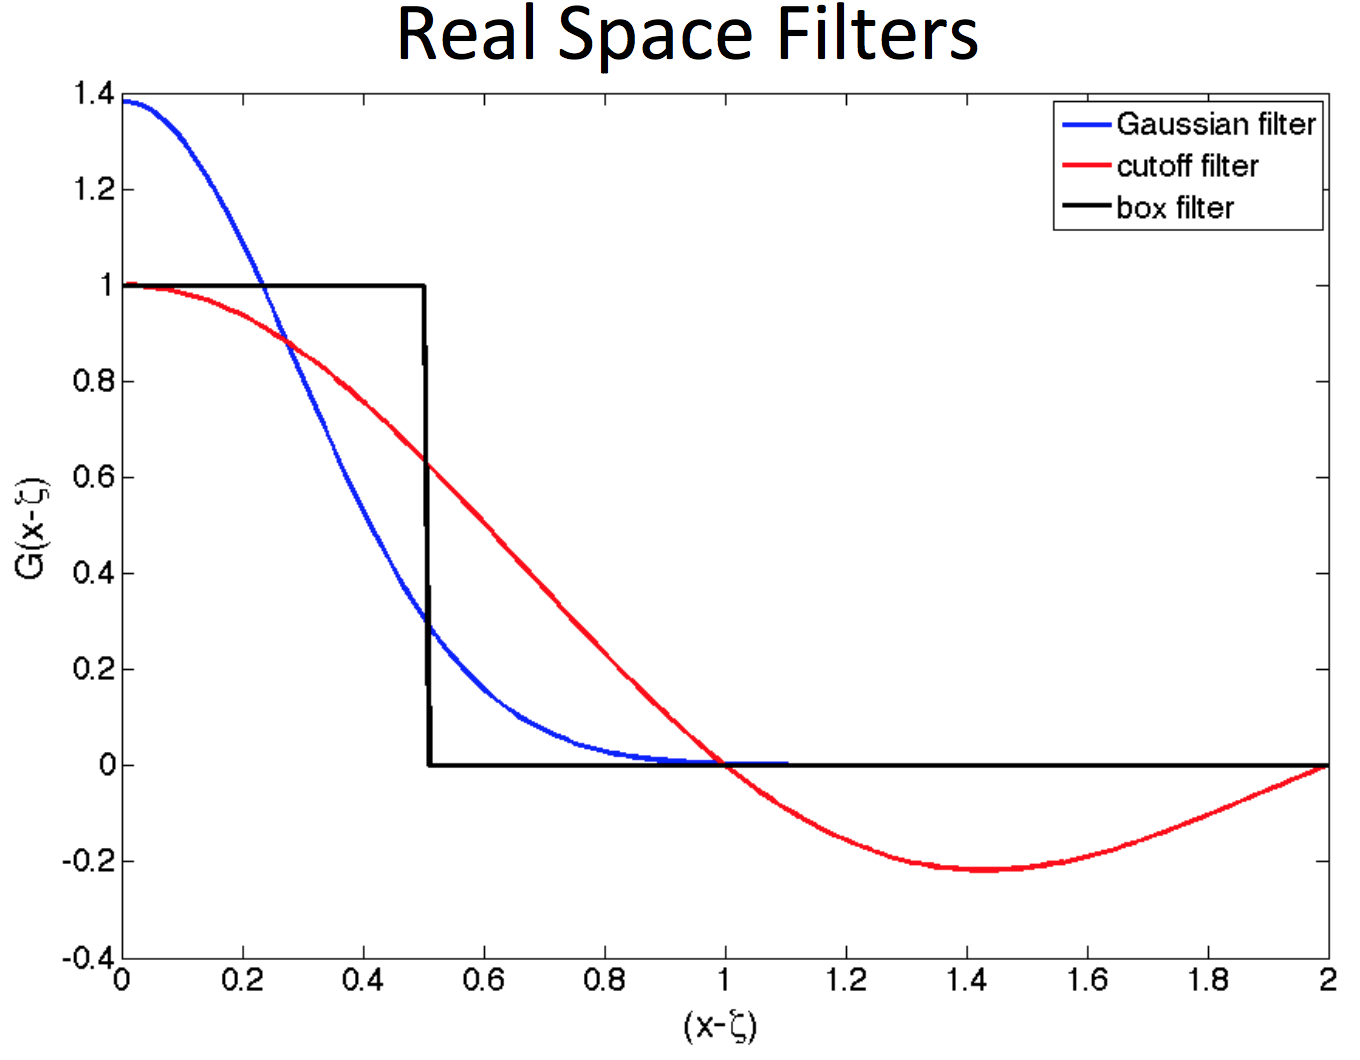
\includegraphics[width=0.5\textwidth]{filter1.png}
	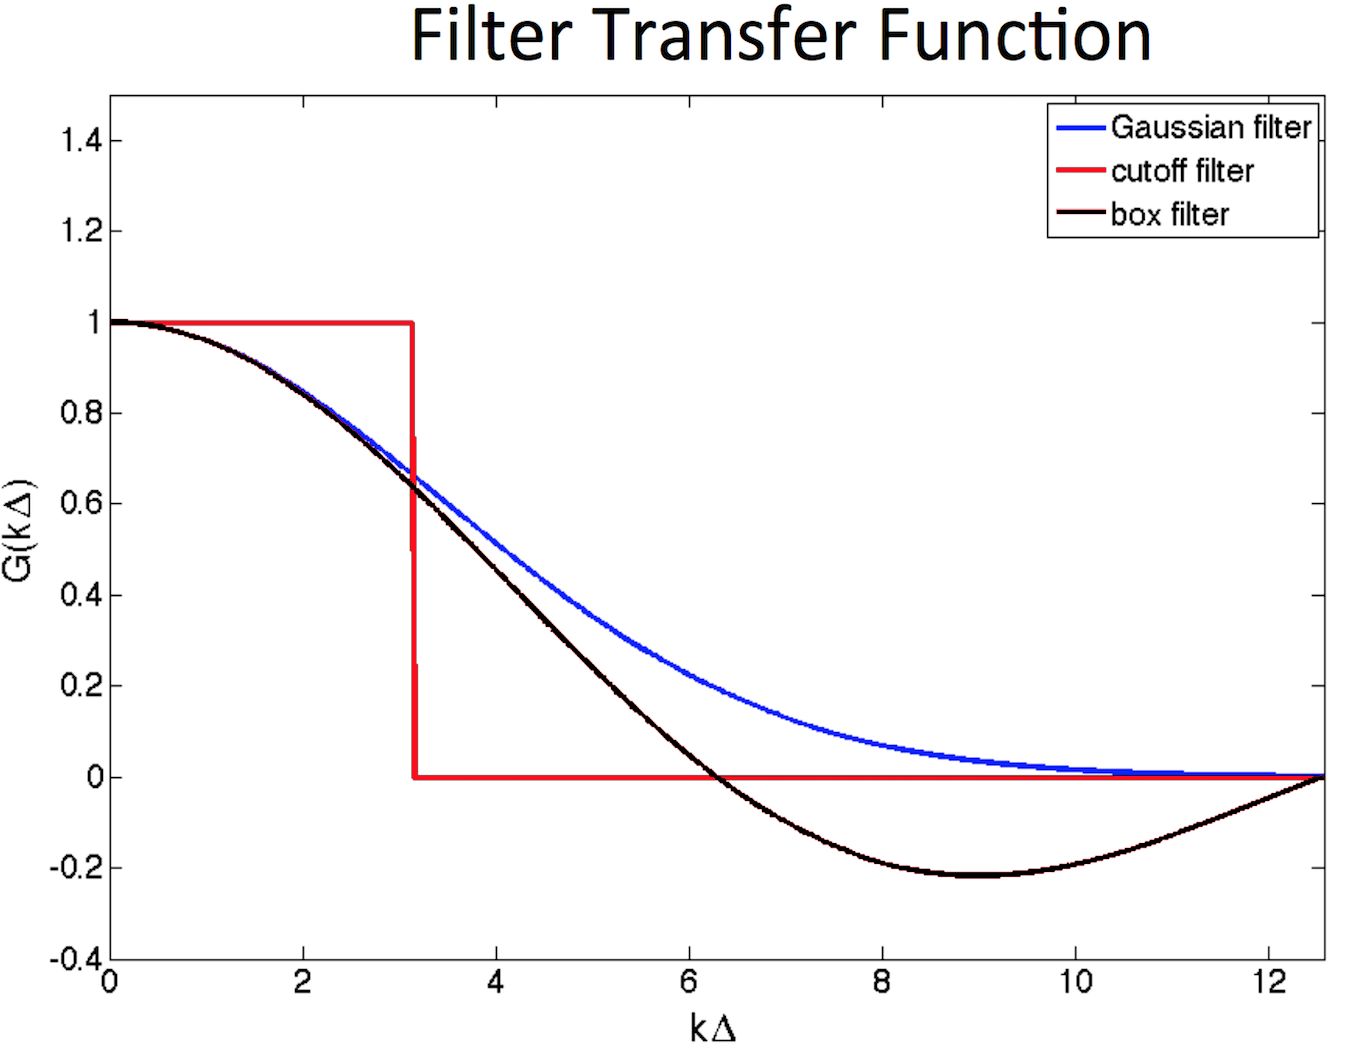
\includegraphics[width=0.5\textwidth]{filter2.png}
\end{figure}
Only the Gaussian filter is local in both real and wave space.
\end{frame}

%------------------------------------------------
\begin{frame}{Filters: local vs non-local}
\begin{itemize}
	\item Where we apply a filter is important.
	\item The Fourier transform of a box filter is a wave, and the inverse transform of a spectral cutoff filter is a wave.
	\item This means we will get different results for these two filters depending on where they are applied.
\end{itemize}
\end{frame}

%------------------------------------------------
\begin{frame}{Filters: local vs non-local}
\begin{itemize}
	\item Thus, we say a box filter is local in physical space and non-local in wavespace.
	\item Conversely, a cutoff filter is local in wavespace and non-local in physical space.
	\item When a filter is non-local, think about it in terms of adding ``wiggles'' everywhere.
	\item As opposed to the box and cutoff filters, the Gaussian filter is (semi) local in both physical space and wavespace (semi because it differs by constants).
	\item This is because the Fourier transform of a Gaussian is also a Gaussian.
\end{itemize}
\end{frame}

%------------------------------------------------
\begin{frame}{Spectral resolution}
\begin{itemize}
	\item We can tie the notion of filters and local/non-local behavior to numerical models and resolution.
	\item The notion of ``spectral'' or ``effective'' resolution arises because the spectra from LES often does not fall at $\Delta$, but rather at some larger scale that is a multiple of $\Delta$.
	\item For instance, a finite difference scheme (perhaps \nth{2}-order central difference) is local in physical space, but non-local in wavespace.
	\item This impacts smaller wavenumbers (larger scales).
\end{itemize}
\end{frame}

%------------------------------------------------
\begin{frame}{Spectral resolution}
\begin{figure}
	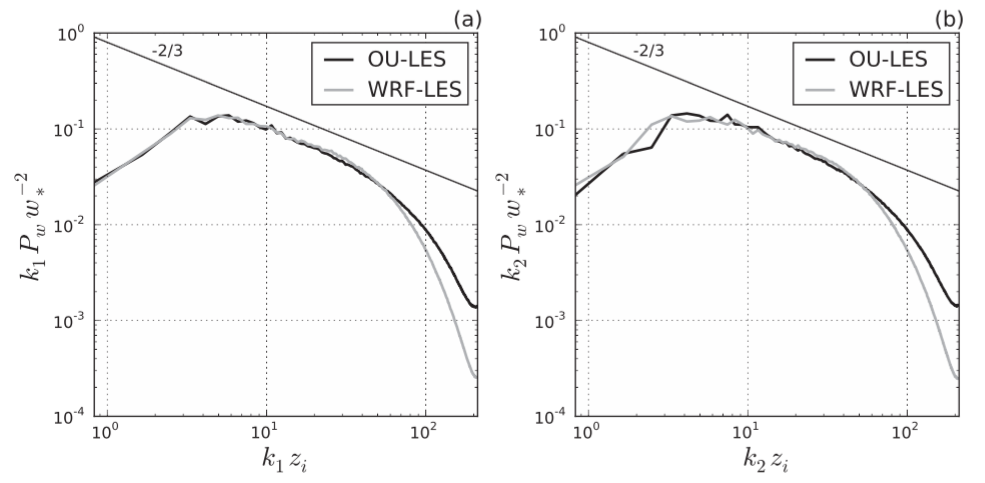
\includegraphics[width=1\textwidth]{effectiveresolution.png}
\end{figure}
From Gibbs and Fedorovich (2014).
\end{frame}

%------------------------------------------------
\begin{frame}{Spectral resolution}
\begin{figure}
	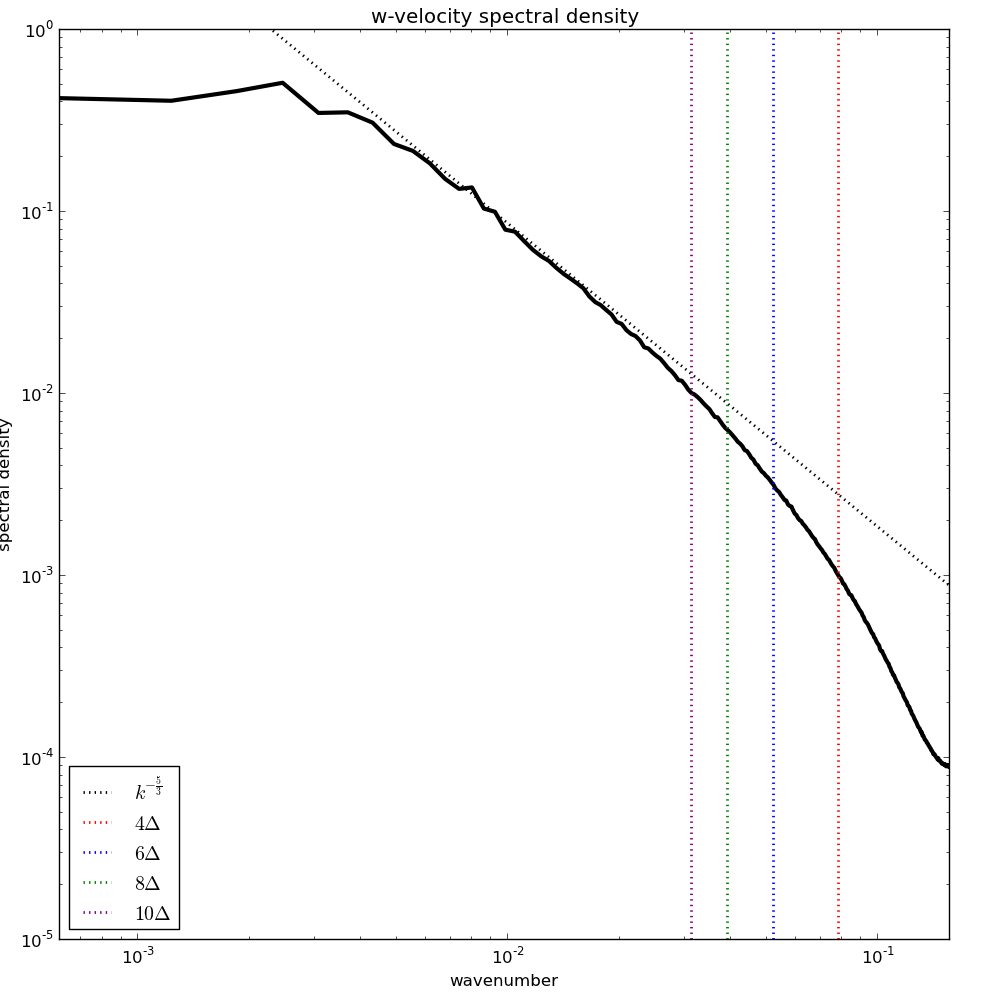
\includegraphics[width=0.75\textwidth]{wspectra.png}
\end{figure}
\end{frame}



%------------------------------------------------
\begin{frame}{Convolution example}
\begin{itemize}
	\item We defined the convolution of two functions as:
	$$\tilde \phi (\vec{x},t) = \int_{-\infty}^{\infty} \phi (\vec{x} - \vec{\zeta},t) G(\vec{\zeta}) d \vec{\zeta}$$
	\item How can we interpret this relation? $G$, our filter kernel, `moves' along our other function $\phi$ and smooths it out (provided it is a low-pass filter).
\end{itemize}
\end{frame}

%------------------------------------------------
\begin{frame}{Convolution example}
\begin{itemize}
	\item One example is using a box filter applied in real space.
	\item See convolution\_example.m (and associated iso\_vel128.mat data file) on Canvas or website.
\end{itemize}
\begin{figure}
	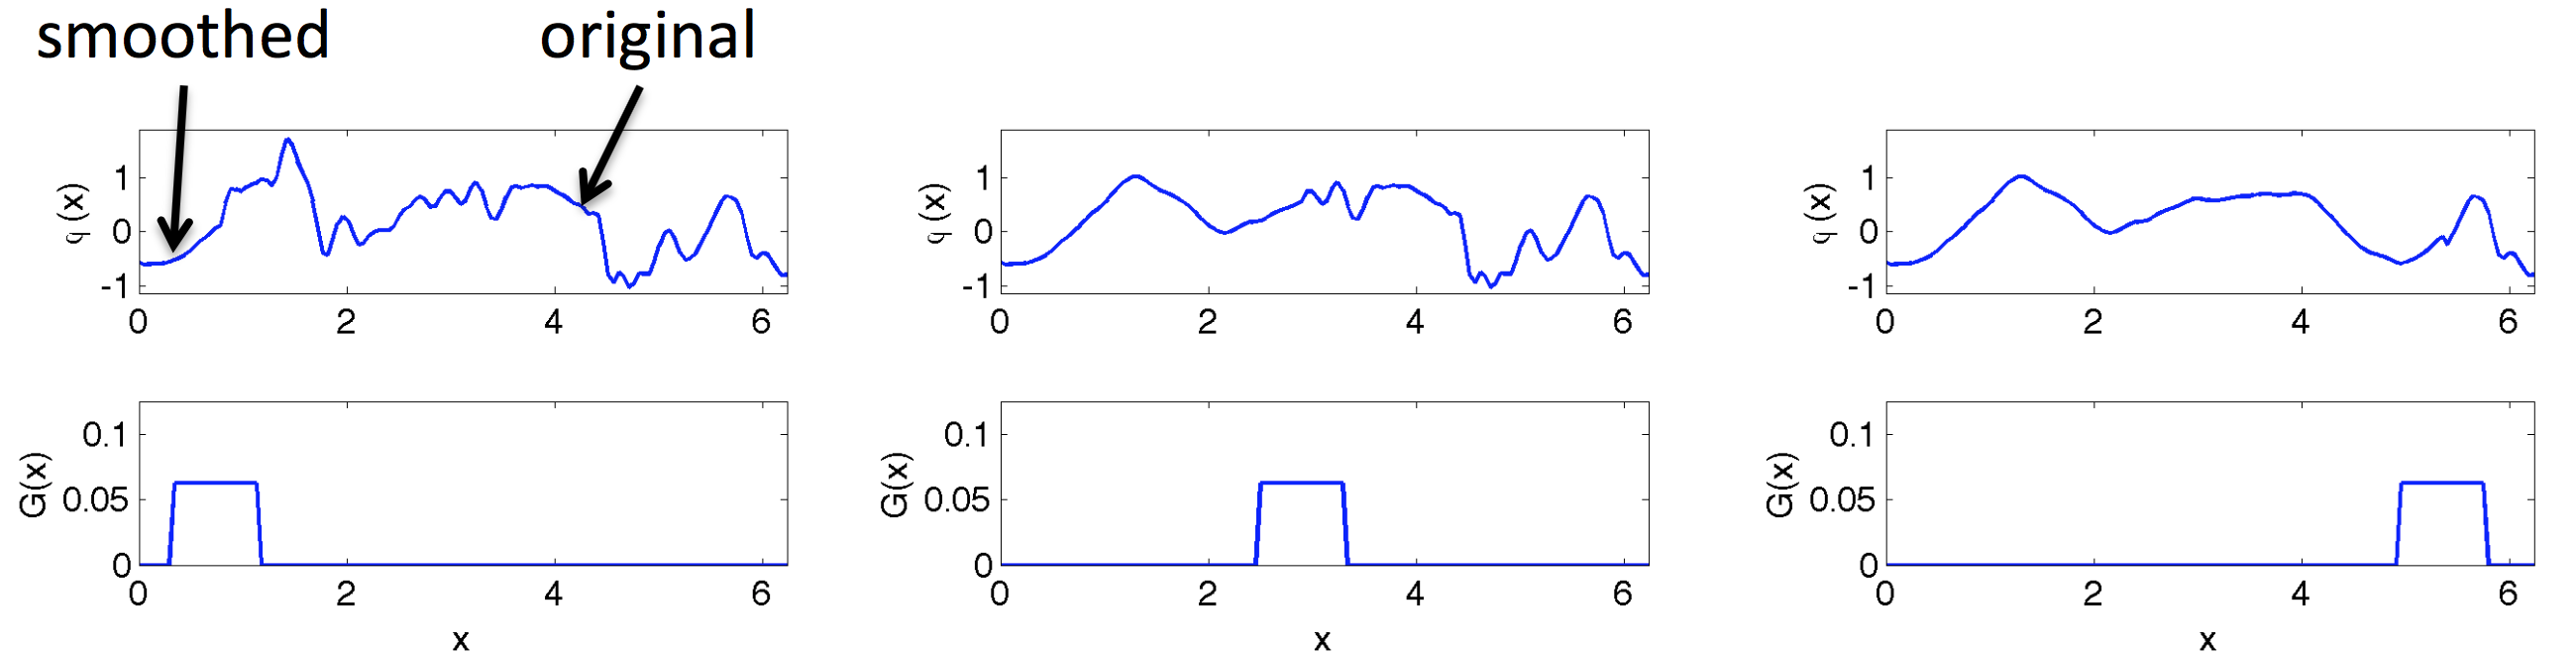
\includegraphics[width=1\textwidth]{convolution.png}
\end{figure}
\end{frame}

%------------------------------------------------
\begin{frame}{Filtering turbulence (real space, cutoff filter)}
\begin{figure}
	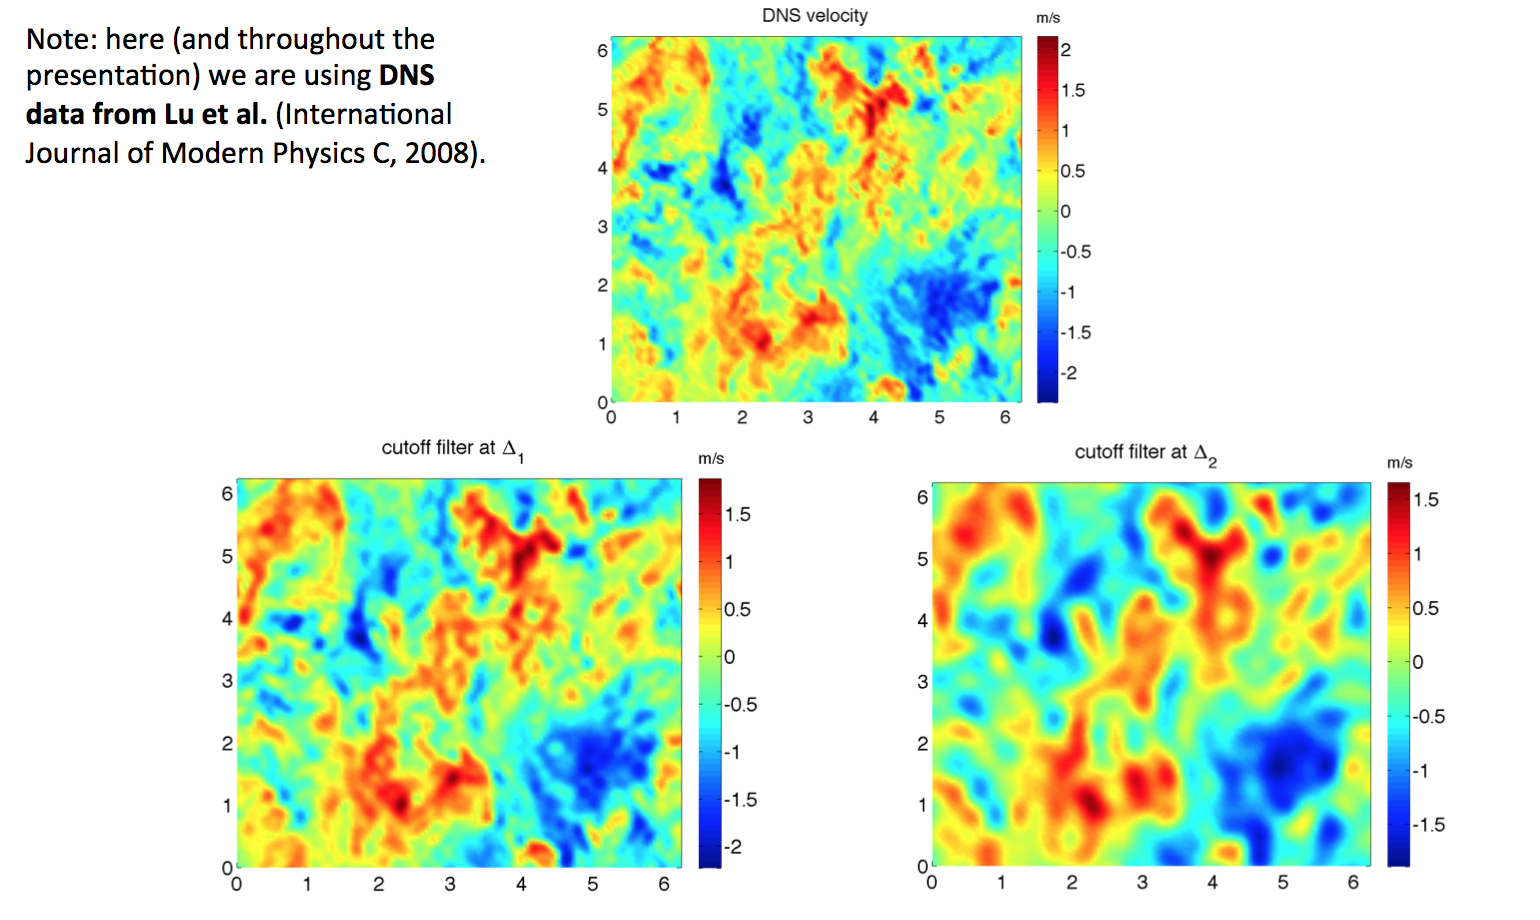
\includegraphics[width=1\textwidth]{filter_cutoff.png}
\end{figure}
\end{frame}

%------------------------------------------------
\begin{frame}{Filtering turbulence (real space, Gaussian filter)}
\begin{figure}
	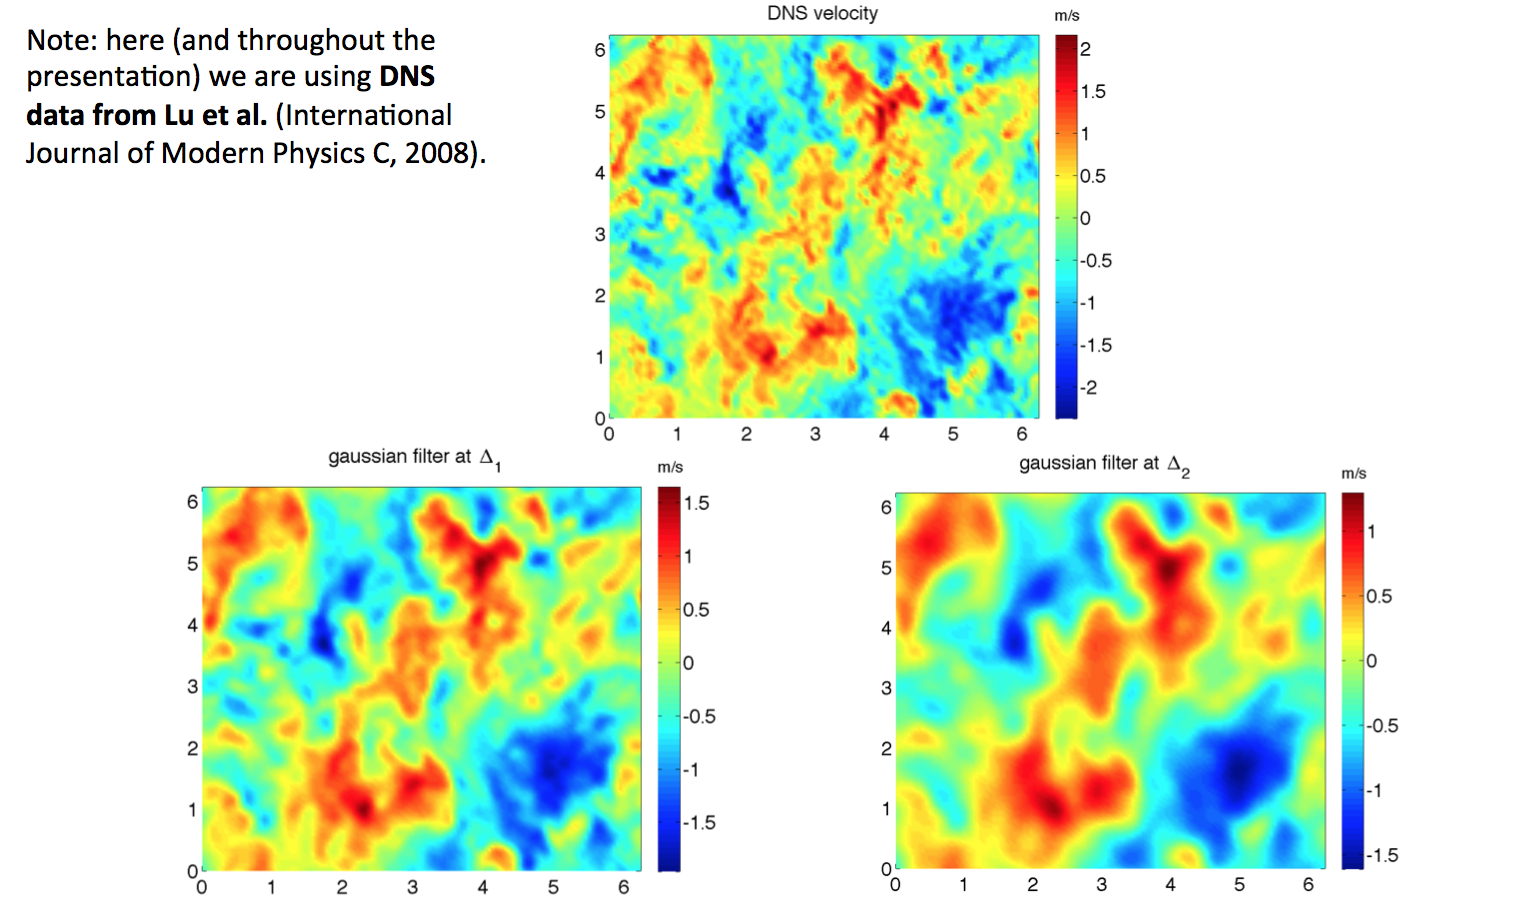
\includegraphics[width=1\textwidth]{filter_gaussian.png}
\end{figure}
\end{frame}

%------------------------------------------------
\begin{frame}{Filtering turbulence (real space, box filter)}
\begin{figure}
	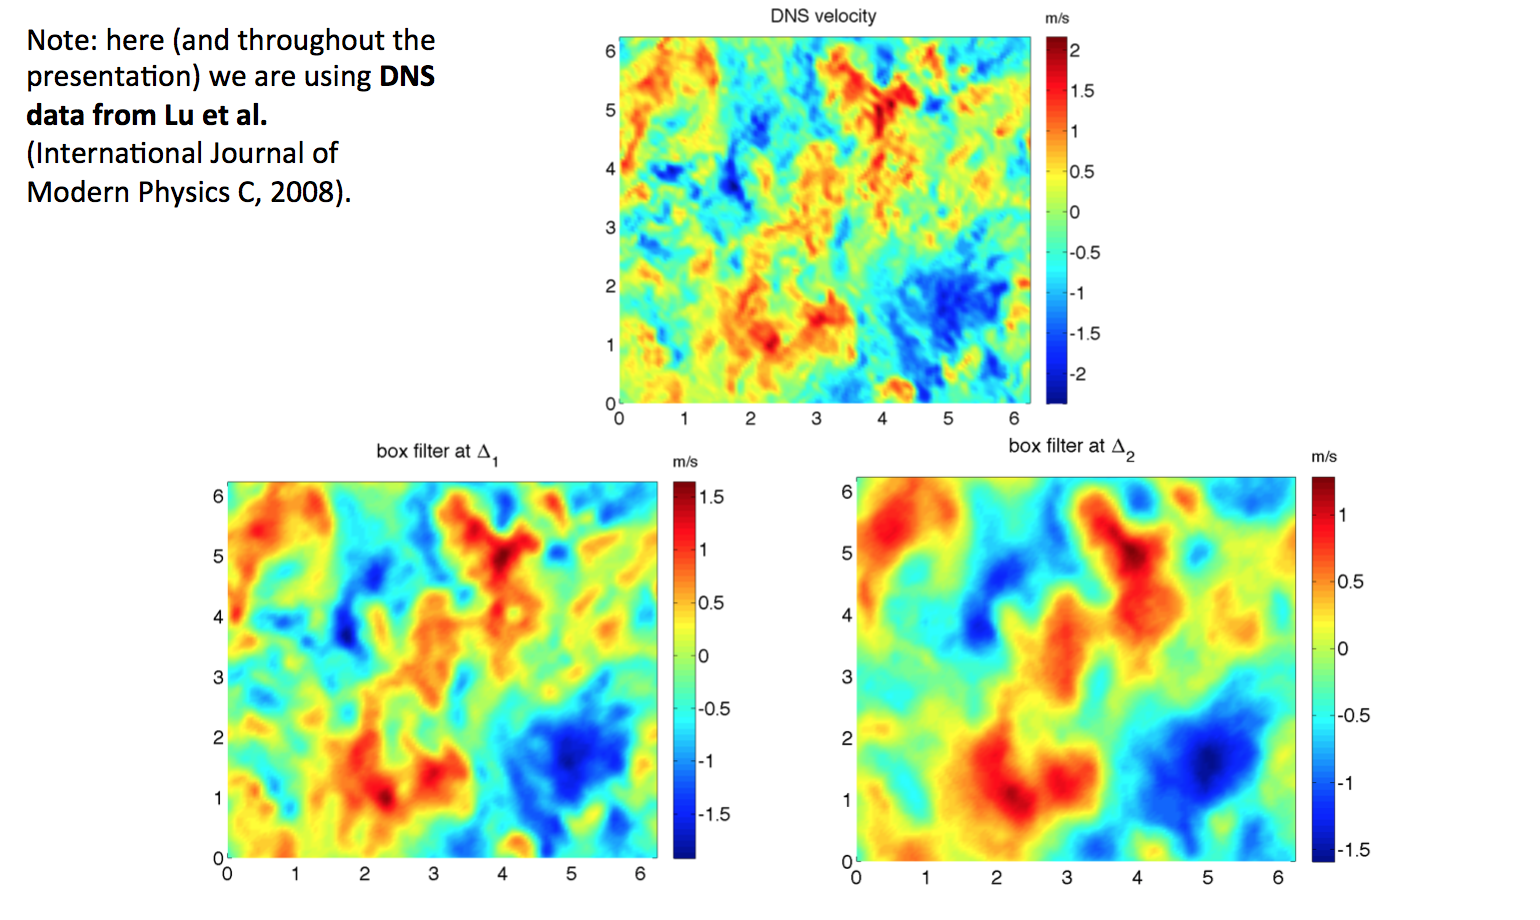
\includegraphics[width=1\textwidth]{filter_box1.png}
\end{figure}
\end{frame}

%------------------------------------------------
\begin{frame}{Filtering turbulence (real space, box filter)}
Another example (Fedorovich and Gibbs, submitted)
\begin{figure}
	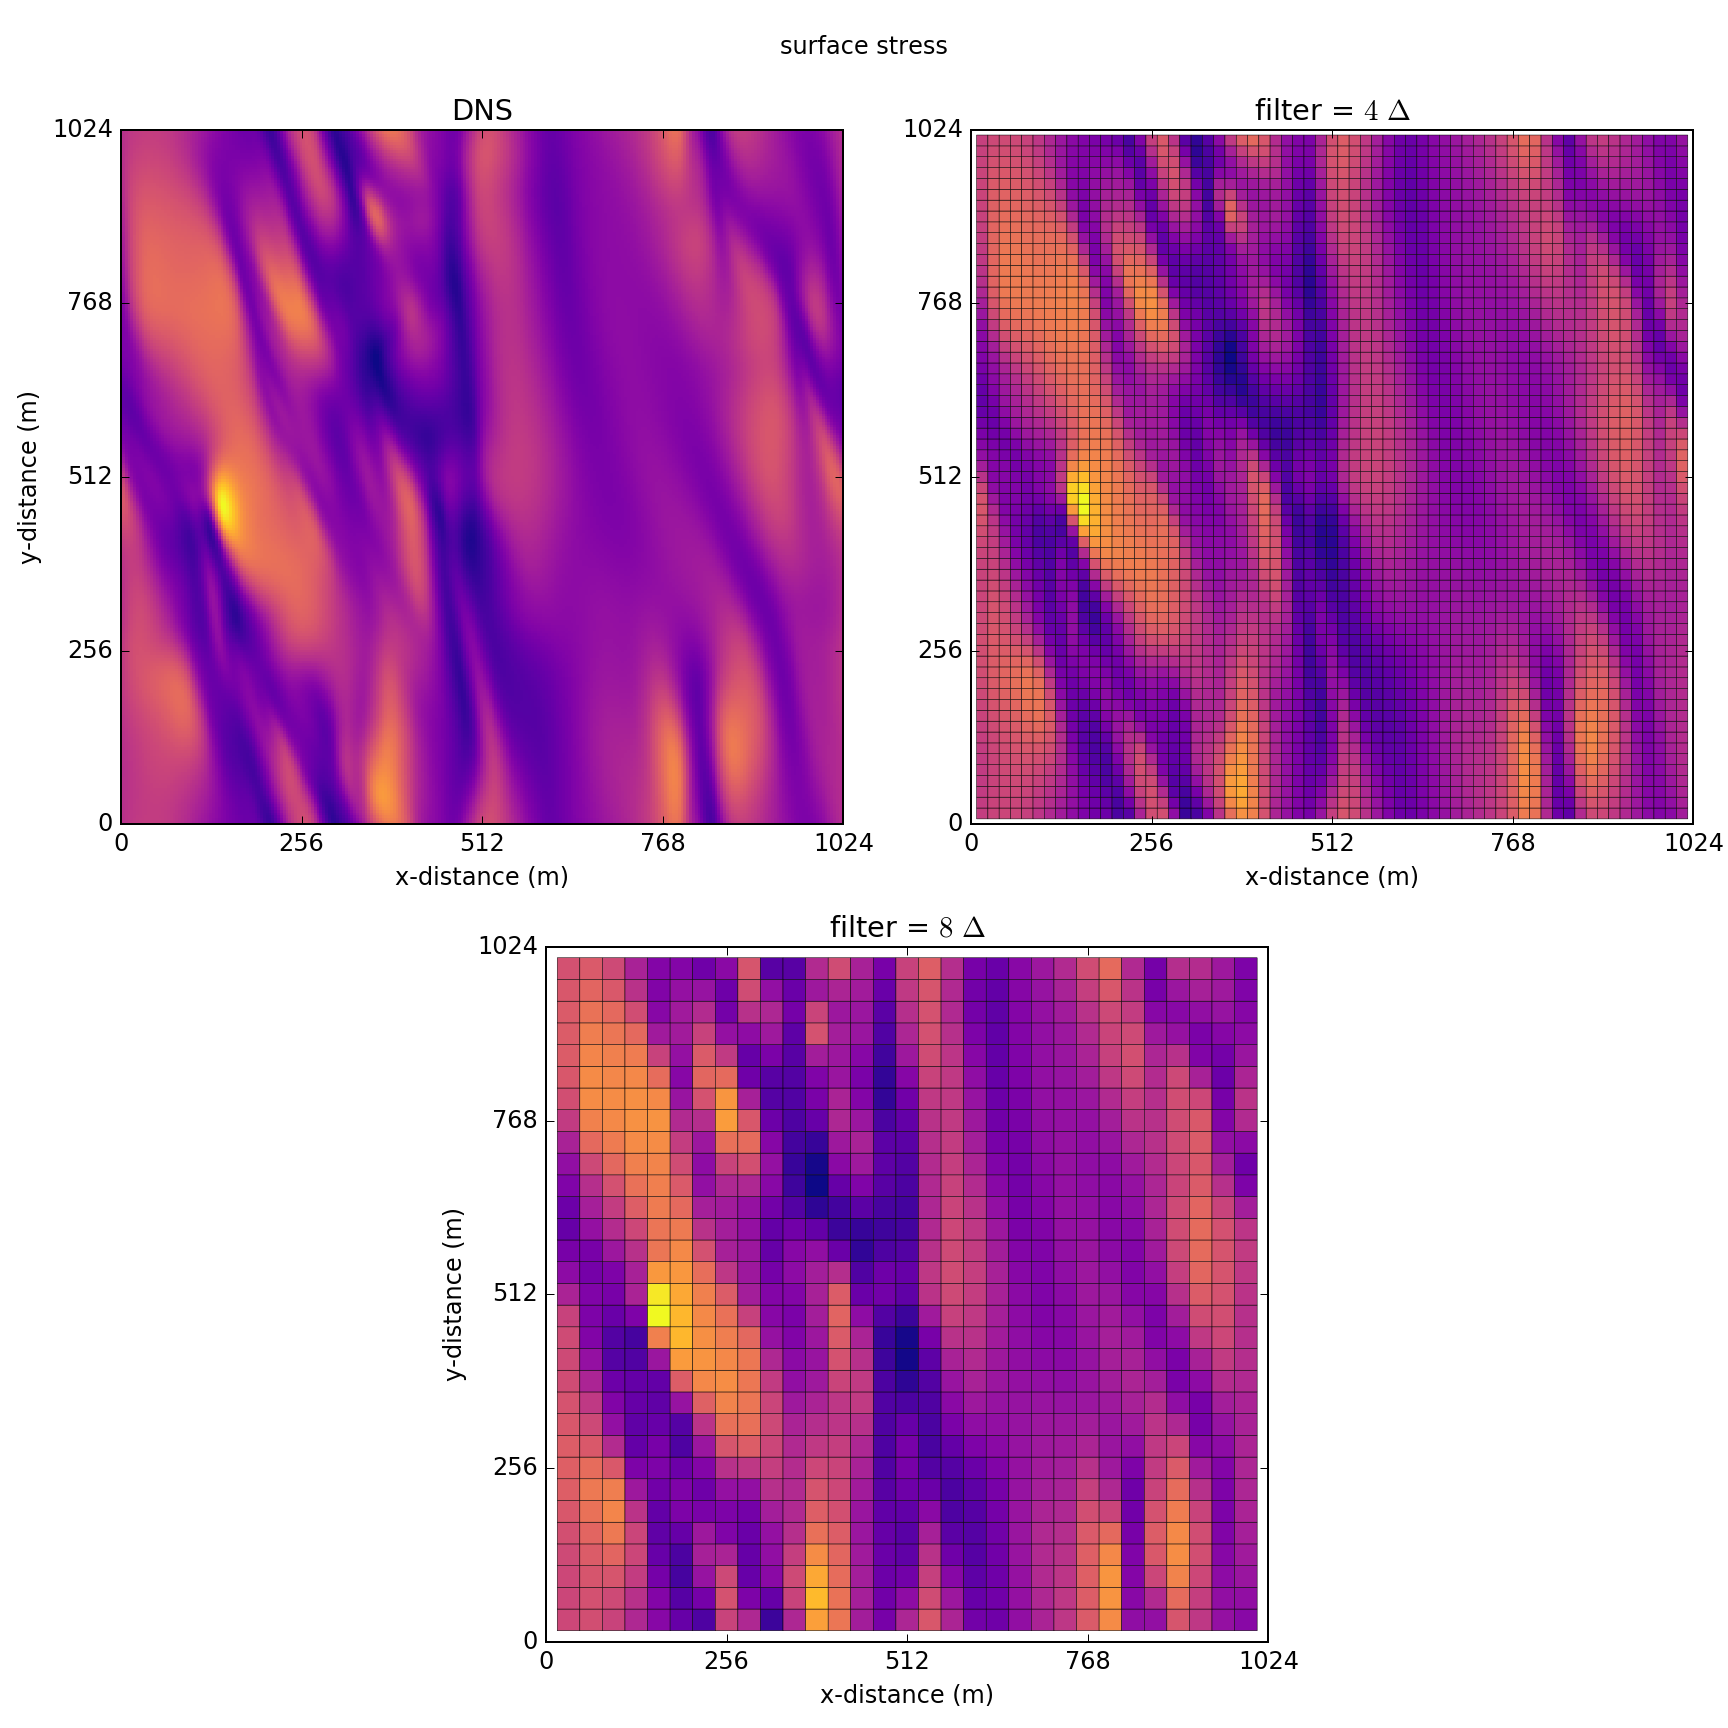
\includegraphics[width=0.7\textwidth]{filter_box2.png}
\end{figure}
\end{frame}

%------------------------------------------------
\begin{frame}{Filtering turbulence (real space)}
\begin{figure}
	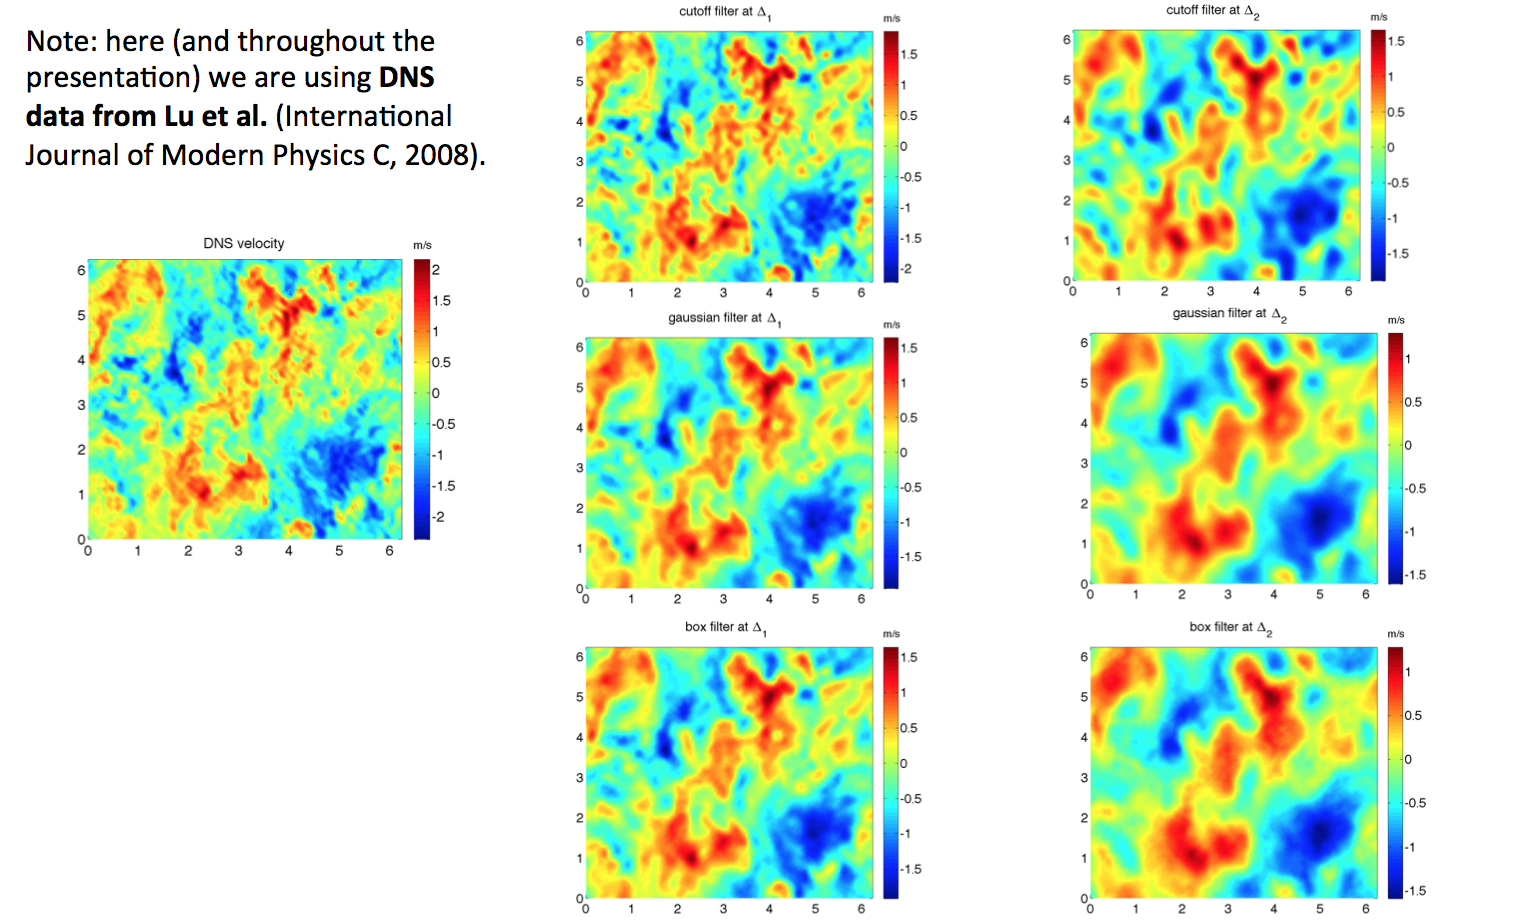
\includegraphics[width=1\textwidth]{filter_all.png}
\end{figure}
\end{frame}

%------------------------------------------------
\begin{frame}{Filtering turbulence (wave space)}
\begin{figure}
	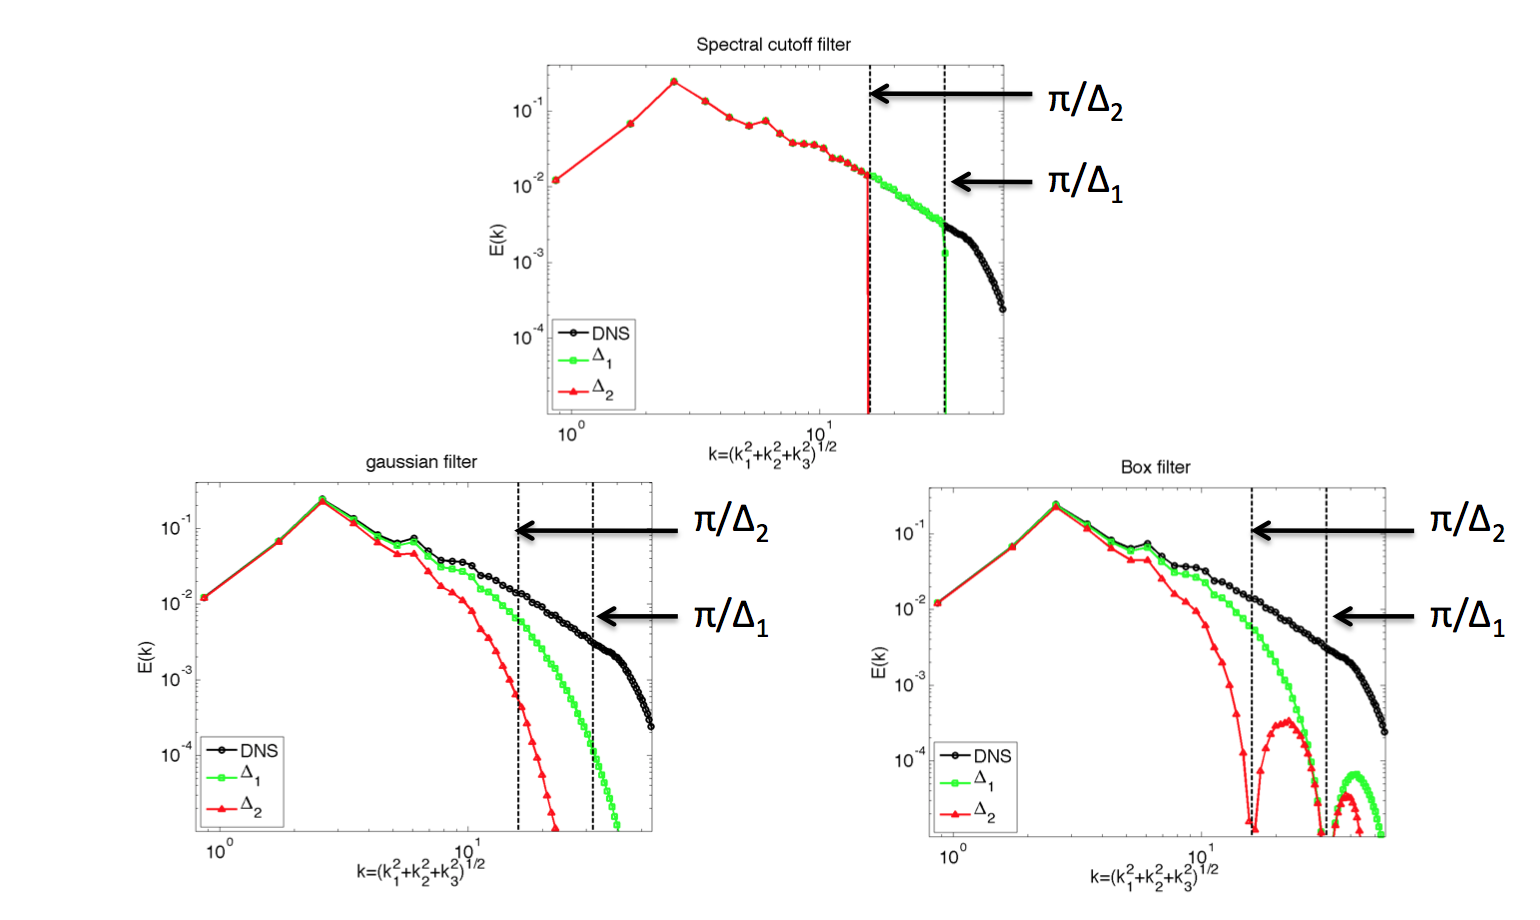
\includegraphics[width=1\textwidth]{filter_wave1.png}
\end{figure}
\end{frame}
%------------------------------------------------
\begin{frame}{Filtering turbulence (wave space)}
\begin{figure}
	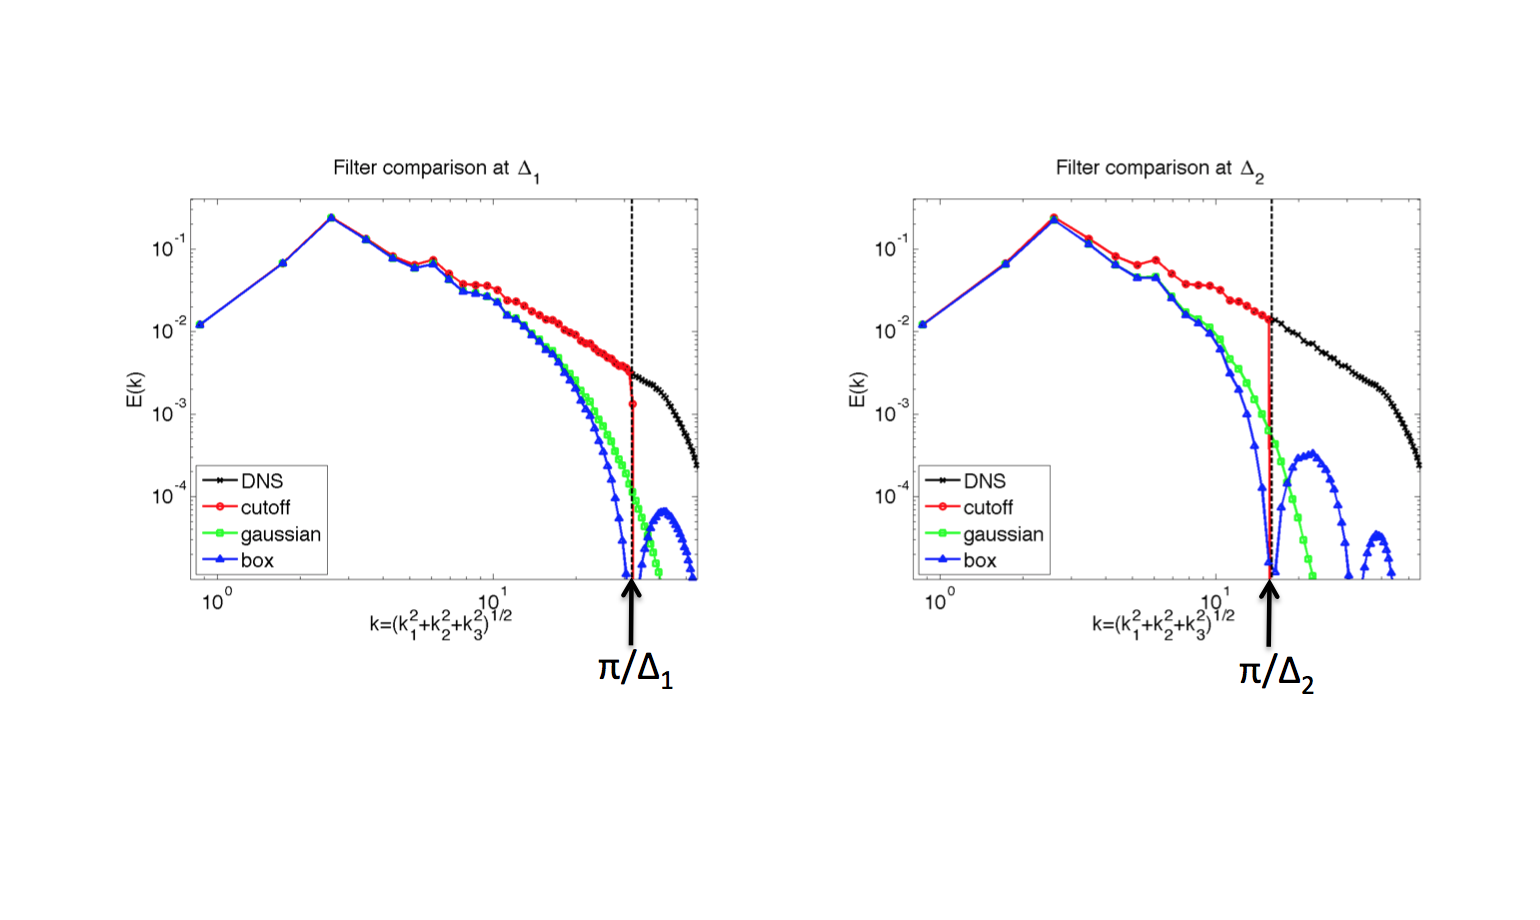
\includegraphics[width=1\textwidth]{filter_wave2.png}
\end{figure}
\end{frame}
%------------------------------------------------
\begin{frame}{Decomposition of turbulence for real filters}

\begin{itemize}
	\item The LES filter can be used to decompose the velocity field into resolved and subfilter scale (SFS) components:
	$$\underbrace{\phi(\vec{x},t)}_{\text{total}} = \underbrace{\tilde \phi (\vec{x},t)}_{\text{resolved}} + \underbrace{\phi^{\prime}(\vec{x},t)}_{\text{subfilter}}$$
	\item We can use our filtered DNS fields to look at how the choice of our filter kernel affects this separation in wavespace.
\end{itemize}
\end{frame}
%------------------------------------------------
\begin{frame}{Decomposition of turbulence for real filters}
\begin{figure}
	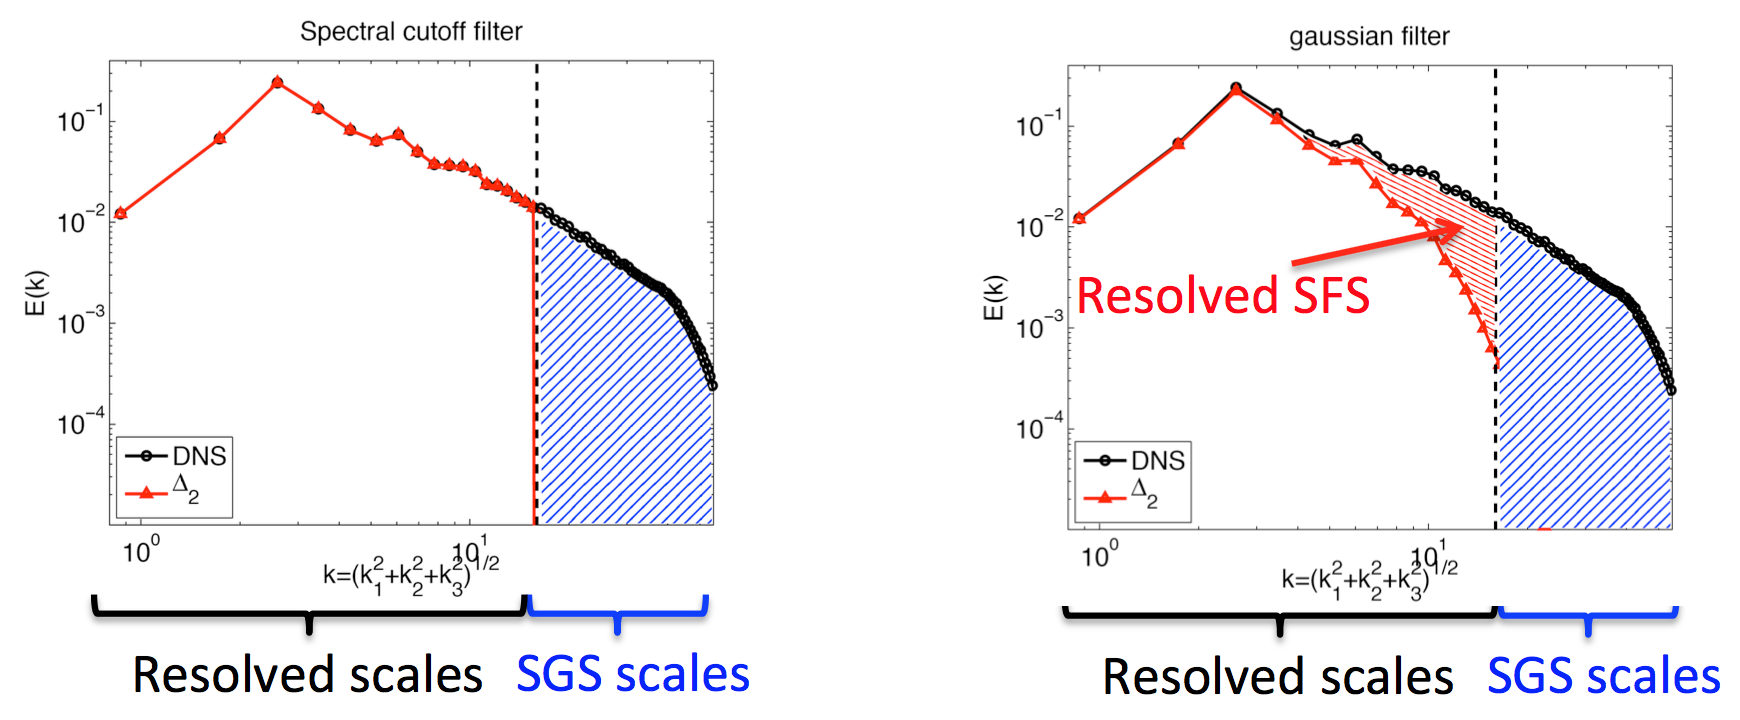
\includegraphics[width=1\textwidth]{filter_decomp.png}
\end{figure}
\begin{itemize}
	\item The Gaussian (or box) filter does not have as compact of support in wavespace as the cutoff filter.
	\item This results in attenuation of energy at scales larger than the filter scale.
	\item The scales affected by the attenuation are referred to as \textit{resolved SFSs}.
\end{itemize}
\end{frame}
%------------------------------------------------



































%------------------------------------------------

\end{document}

